\documentclass{beamer}
\usepackage{tabularx}
\usepackage{booktabs}

% Frankfurt <3
\usetheme{Frankfurt}

% Some basic stuff for the first slide
\title{Making recommendations using extremely sparse
       implicit datasets}
\subtitle{SoBazaar Workshop}
\date{2014-06-10}
\author{Martin Christian Havig, Thomas Almenningen \& Herman Schistad}

\begin{document}

  % Title page, showing title, date and authors.
  \begin{frame}
    \titlepage
  \end{frame}

  % Kickstart stuff with e-commerce statistics and competitor overview
  \begin{frame}
    \frametitle{E-commerce in Norway since 2005}
  \end{frame}

  \begin{frame}
    \frametitle{Competitor Overview}
  \end{frame}

  % The table of contents, showing sections and subsections.
  \begin{frame}
    \frametitle{Structure}
    \tableofcontents
  \end{frame}

  % First section concerns the data and general overview of application
  \section{Data analysis and application overview}

  % Some key figures and what they mean.
  \begin{frame}
    \frametitle{SoBazaar Data - Dataset Summary}
      \begin{table}[H]\centering\resizebox{\columnwidth}{!}{\begin{tabular}{*{19}l}
        \centering
        \begin{tabular}{l l}
            \toprule
            Attribute       & Count   \\
            \midrule
            Total number of events  &    218975 \\
            Unique users ids    &    2021 \\
            Unique item ids     &    6092 \\
            Unique storefronts  &    147 \\
            Unique retailer brands  &    24 \\
            \hline
            First event & Mon, 07 Oct 2013 10:59:57 GMT \\
            Last event & Mon, 19 May 2014 22:51:19 GMT \\
            Lifetime of data & 224 days \\
            \hline
            Item clicks     &    25491 \\
            Item wants   &    13262 \\
            Item purchases   &    2020 \\
            \hline
            Average item click count per user   &    12.6130 \\
            Average item want count per user     &    6.5620 \\
            Average item purchase count per user     &    0.9995 \\
            \hline
            Average item interaction count per user     &    20.1746 \\
            Average user interaction count per item     &    6.6928 \\
            \bottomrule
        % \caption[Dataset summary]{Overview of the key figures in the SoBazaar dataset}
        % \label{table:datasetSummary}
        \end{tabular}
    \end{table}
\bottomrule\end{tabular}}\caption{time mahout-itembased}\end{table}
  \end{frame}

  % Continuation of key figures w/ visualizations.
  \begin{frame}
    \frametitle{SoBazaar Data - Something else}
    % \begin{figure}[H]
    %     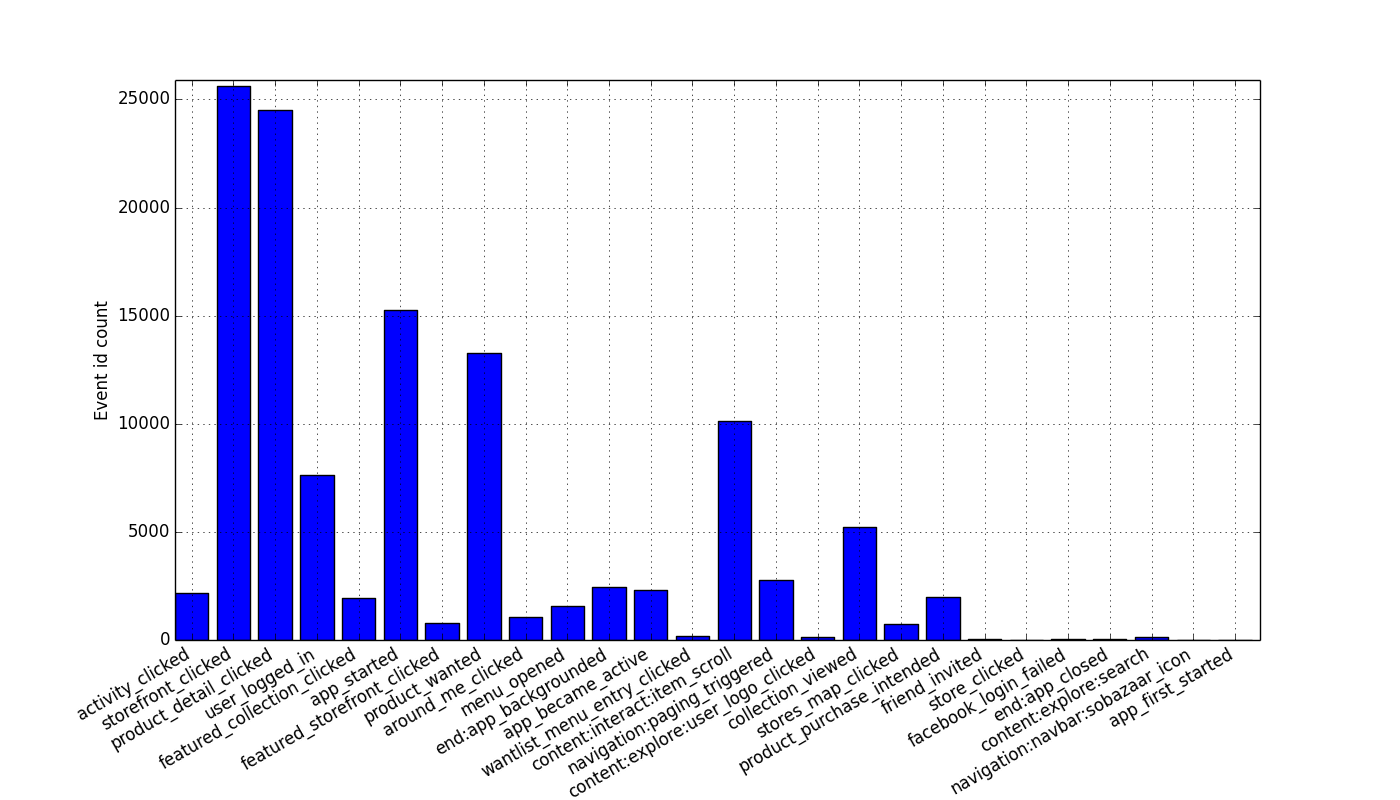
\includegraphics[width=5in]{../src/image/event_iddistribution.png}
    %     \centering
    %     \caption{Event distribution}
    % \label{figure:eventIDDistribution}
    % \end{figure}
    \begin{itemize}
      \item
    \end{itemize}
  \end{frame}

  % What does it mean that feedback is implicit?
  \begin{frame}
    \frametitle{Implicit feedback}
    \begin{itemize}
      \item
    \end{itemize}
  \end{frame}

  % How we propose to recommend items for SoBazaar
  \begin{frame}
    \frametitle{Application Overview}
  \end{frame}

  % Second section, going through each of these components.
  \section{Proposed system components}

  % Component one: creating implicit ratings.
  \begin{frame}
    \frametitle{Converting Implicit Feedback}
    \begin{itemize}
      \item
    \end{itemize}
  \end{frame}

  % Component two: filterbots and cold-start stuff.
  \begin{frame}
    \frametitle{Cold start boosting}
    \begin{itemize}
      \item
    \end{itemize}
  \end{frame}

  % Component three: actually making recommendations.
  \begin{frame}
    \frametitle{Making recommendations}
    \begin{itemize}
      \item
    \end{itemize}
  \end{frame}

  % Component four: how to evaluate the results.
  \begin{frame}
    \frametitle{Evaluation}
    \begin{itemize}
      \item
    \end{itemize}
  \end{frame}

  % Section three: a summary and conclusions from our work.
  \section{Results and future work}

  % Some thoughts on what we have found.
  \begin{frame}
    \frametitle{Conclusions}
    \begin{itemize}
      \item
    \end{itemize}
  \end{frame}

  % Figure showing system in relation to "the sky".
  \begin{frame}
    \frametitle{How to implement in SoBazaar}
    \begin{itemize}
      \item
    \end{itemize}
  \end{frame}

  % How can future results be improved?
  \begin{frame}
    \frametitle{Improving results}
    \begin{itemize}
      \item Better results can be achieved with using Tinder-like interface.
      \item Framework for online evaluation
    \end{itemize}
  \end{frame}

\end{document}
